\documentclass[conference]{IEEEtran}
\IEEEoverridecommandlockouts

\usepackage{cite}
\usepackage{amsmath,amssymb,amsfonts}
\usepackage{algorithmic}
\usepackage{graphicx}
\usepackage{textcomp}
\usepackage{xcolor}

\usepackage[T1]{fontenc}
\usepackage[utf8]{inputenc}
\usepackage{subcaption}
\usepackage{siunitx}
\usepackage[hidelinks]{hyperref}

\def\BibTeX{{\rm B\kern-.05em{\sc i\kern-.025em b}\kern-.08em
    T\kern-.1667em\lower.7ex\hbox{E}\kern-.125emX}}
\begin{document}

\title{\large Exposé: Implementierung eines In-Memory Key-Value Stores auf Basis von optimierten B\textsuperscript{+}-Bäumen}

\author{\IEEEauthorblockN{Janne Gruhler, Maxim Bellm, Albert Rico Martin, Matthias Raba}
\IEEEauthorblockA{Department of Computer Science -- Hochschule Furtwangen -- Furtwangen, Germany}
}

\maketitle
\renewcommand{\figureautorefname}{Abb.}

\section{Einführung und Motivation}

B\textsuperscript{+}-Bäume zählen zu den grundlegendsten Indexstrukturen in Datenbanksystemen,
galten für In-Memory-Szenarien aber lange als unterlegen: Systeme wie Redis setzen auf
hash-basierte Strukturen mit nahezu konstanter Latenz pro Zugriff.
Das Paper \emph{``B-trees are back: Engineering fast and pageable node layouts''}
von Müller, Benson und Leis~\cite{muller2025b} zeigt, dass dies vor allem
implementierungsbedingt ist. Durch mehrere Knotentypen, Fingerprinting, Hinting,
Präfixkompression und SIMD-Beschleunigung erreichen B\textsuperscript{+}-Bäume
vergleichbaren Durchsatz wie der Adaptive Radix Tree~(ART) und der Height Optimized Trie~(HOT).
Ziel dieses Projekts ist es, diese Ergebnisse nachzuvollziehen und einen eigenen,
Redis-kompatiblen Key-Value Store auf dieser Basis zu implementieren.

\section{Analyse und Modernisierung des Repositories}

Der Code des Papers ist öffentlich auf GitHub verfügbar, war aber stark auf eine spezifische
Compilerumgebung zugeschnitten. SIMD-Intrinsics waren direkt als AVX2-Code eingebettet
und das Build-System bestand aus einem handgeschriebenen, monolithischen Makefile.
Wir haben das Repository in eine statische Bibliothek (\texttt{libbtree}) umgebaut.
Dazu haben wir das Build-System auf CMake migriert, die SIMD-Logik hinter
plattformunabhängigen Abstraktionen gekapselt und den Code auf modernes C++ aktualisiert.
Eine einheitliche \texttt{DataStructureWrapper}-Schnittstelle macht die Bibliothek
einfach in andere Projekte einbindbar.

\section{Nachvollziehen der Messergebnisse}

Die Benchmarks des Papers laufen über Python-Skripte, die Benchmarkingprogramme
mit Parametern wie Schlüsselanzahl, Operationsanzahl und Batchgröße aufrufen,
Ergebnisse als CSV speichern und in R visualisieren. Als Datensätze kamen dichte
und dünn besetzte Integer-Schlüssel, Wikipedia-Artikeltitel und zufällig generierte
URLs zum Einsatz.
Das Nachvollziehen war aufwändig: Die verwendeten Datensätze sind nur im Paper
beschrieben, nicht im Repository beigelegt. Wir mussten sie selbst generieren, was
die Vergleichbarkeit einschränkt. Nicht alle Grafiken ließen sich eindeutig einem
Skript zuordnen, und unsere Messwerte wichen teils um Größenordnungen von den
publizierten Werten ab. Nach Kontaktaufnahme mit einem der Autoren bekamen wir
Zugriff auf die Originaldatensätze. Der Autor bestätigte, dass einige Messungen
unter schwer reproduzierbaren Bedingungen entstanden sind.

\section{Implementierung eines Redis-kompatiblen Key-Value Stores}

Auf Basis von \texttt{libbtree} haben wir in C++ einen Key-Value Store gebaut,
der das Redis Serialization Protocol~(RESP) spricht und damit als Drop-in-Ersatz
für Redis eingesetzt werden kann. Die Netzwerkschicht basiert auf Boost.Asio.
Unterstützt werden die gängigen Kommandos \texttt{GET}, \texttt{SET}, \texttt{MGET},
\texttt{MSET}, \texttt{DEL}, \texttt{EXISTS}, \texttt{INCR}/\texttt{DECR} und \texttt{INFO}.
Zum Vergleich haben wir YCSB2 genutzt, das eine identische Last gegen beide Server richtet.
Verwendet wurde Workload~C (100\,\% Lesezugriffe, Zipf-verteilt) über
Batch-\texttt{MGET}-Anfragen. \autoref{fig:benchmark} zeigt den Durchsatzvergleich nach Datenbankgröße.
Ab ca.\ \num{500000} Einträgen ist unser System kompetitiv. Bei kleineren Datenmengen
überwiegt der Aufbauoverhead des Baums gegenüber Redis's O(1)-Hash-Lookups. Ein struktureller Vorteil von B\textsuperscript{+}-Bäumen ist die geordnete Schlüsselspeicherung,
die Range-Scans ohne zusätzliche Datenstrukturen ermöglicht. Bei Redis ist das nicht möglich,
da Hashing grundsätzlich keine Ordnung beibehält.

\begin{figure}[htbp]
    \centering
    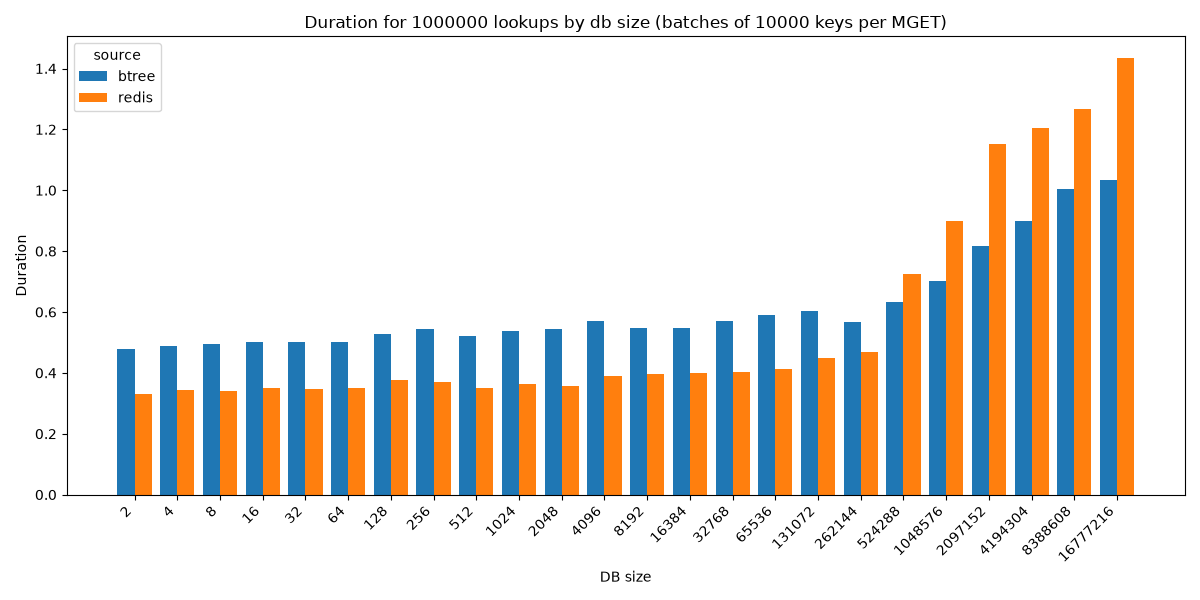
\includegraphics[width=\linewidth]{img/mget.png}
    \caption{YCSB2 Workload~C: Durchsatz btree-redis vs.\ Redis nach Datenbankgröße.}
    \label{fig:benchmark}
\end{figure}

\section{Fazit}

Die im Paper beschriebenen optimierten B\textsuperscript{+}-Bäume sind neben disk-basierten Datenbanken eine solide Grundlage für wettbewerbsfähige In-Memory Key-Value Stores. Die Messergebnisse des Papers konnten nur teilweise reproduziert werden, was
zeigt, wie wichtig eine saubere experimentelle Dokumentation in der Systemforschung ist.

\nocite{*}
\bibliographystyle{IEEEtran}
\bibliography{sources}

\end{document}
